\documentclass[12pt]{article}
\usepackage{amsmath}
\usepackage{graphicx}
\title{Report for Auto Control Lab12}
\date{2020/12/8}
\author{Jacky Yeh 4107064003}

\begin{document}
\begin{titlepage}

\maketitle
\end{titlepage}


\section{Introduction}
This is the Experiment of Auto Control Lab where TAs taught us the plot of root locus and the identification of desired K value to keep the system under stable.Also with other specified values including the settling time and percent overshoot.


\section{LAB12}
\subsection{Part 1 Homework problems and its codes}
Objective:Draw the root locus with code\\
These are the stated Homework problems\\
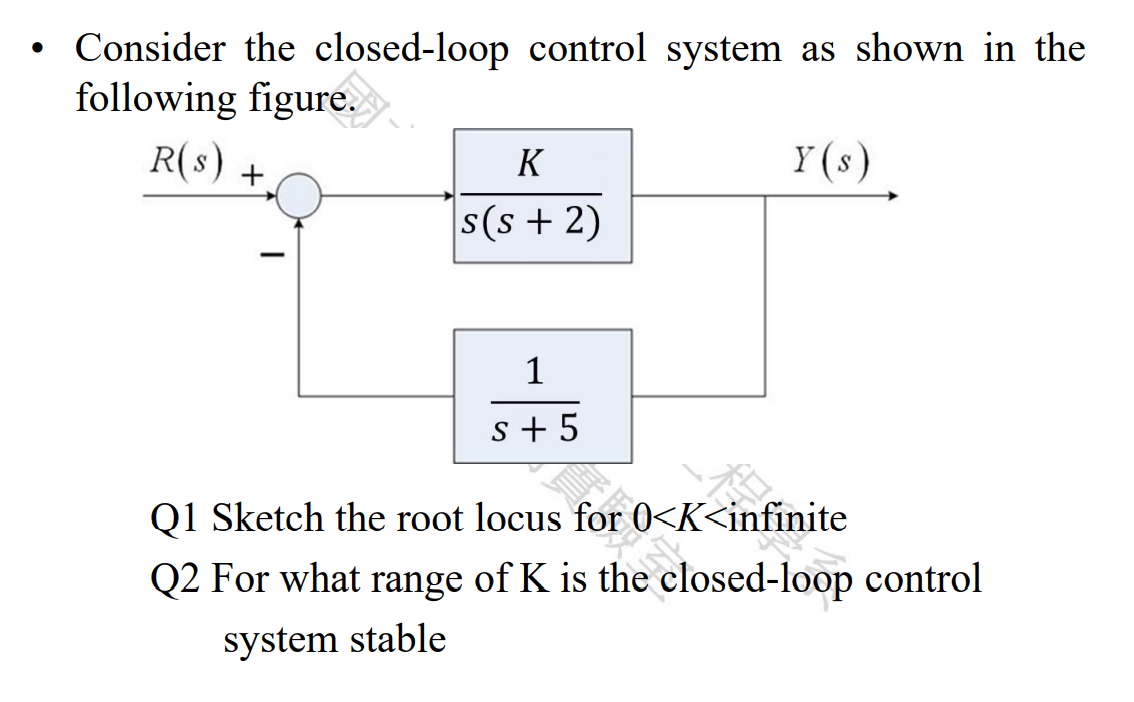
\includegraphics[scale=0.5]{../Lab12/Problem1.png}\\ 

\cleardoublepage
\subsection{CODES FOR PROBLEM1}
In order to perform the tasks, Matlab codes are needed. The following is the code needed for plotting\\

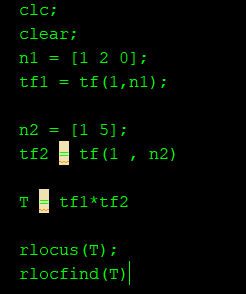
\includegraphics[scale=2]{../Lab12/Code1.png}\\ 

\subsection{Result of the Code desire gain} 

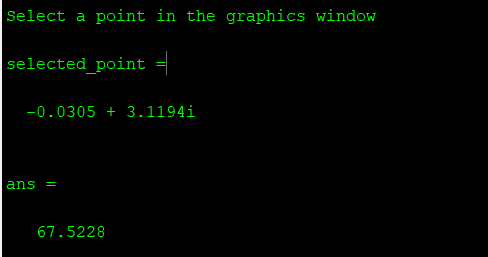
\includegraphics[scale=1]{../Lab12/ResultofK.png} \\
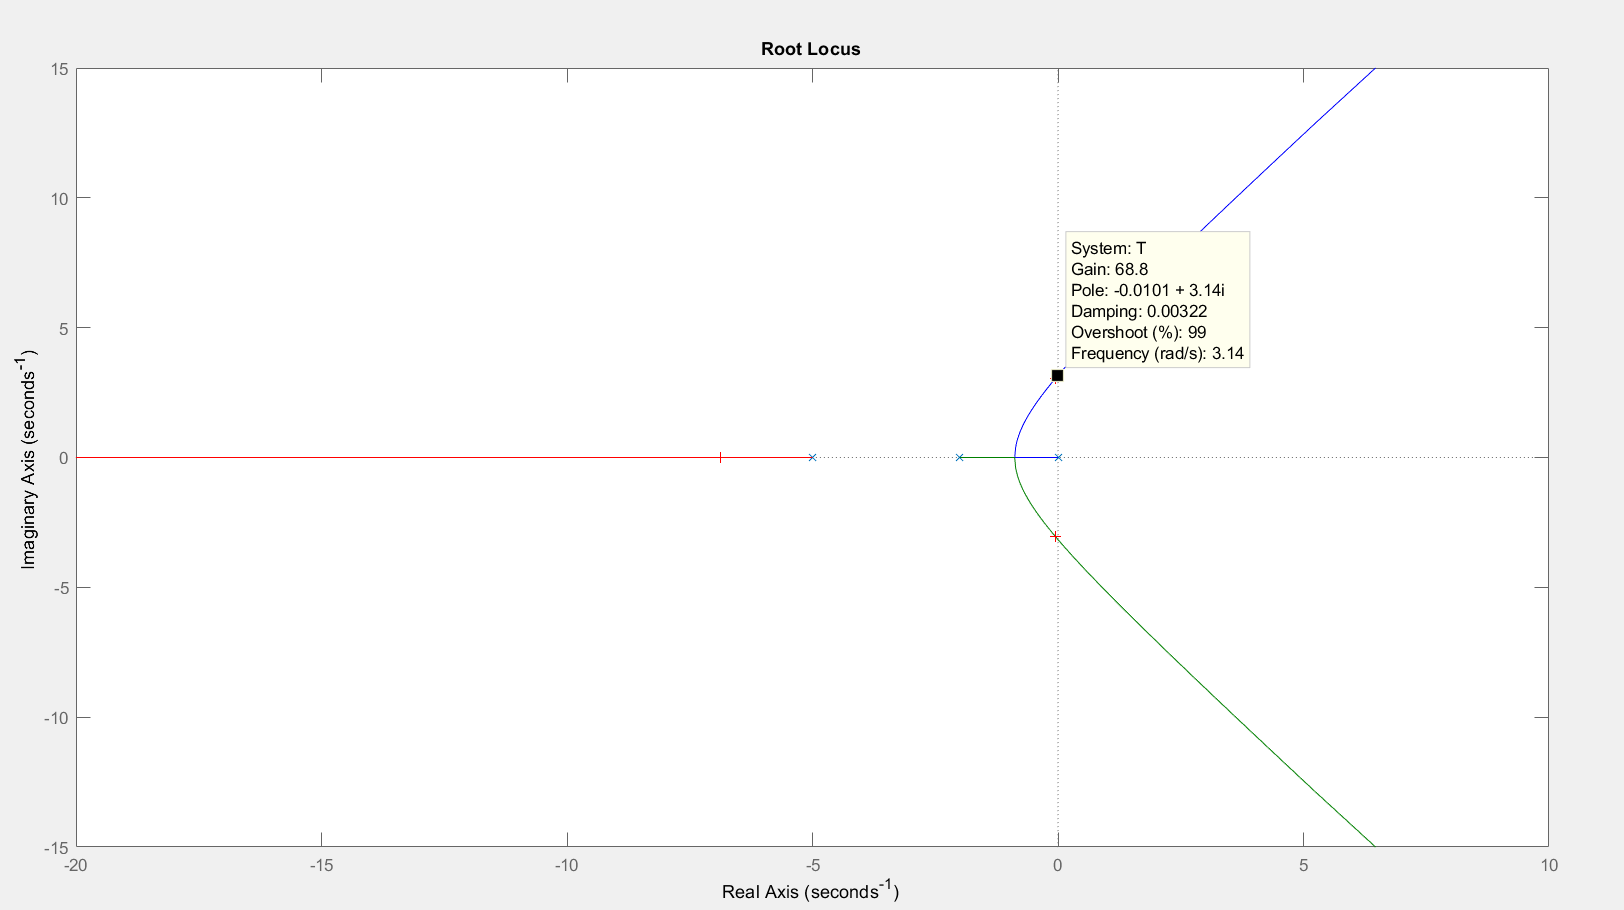
\includegraphics[scale=0.5]{../Lab12/Result1.png}\\


\cleardoublepage

 
\subsection{Part 2 Homework problems and codes}

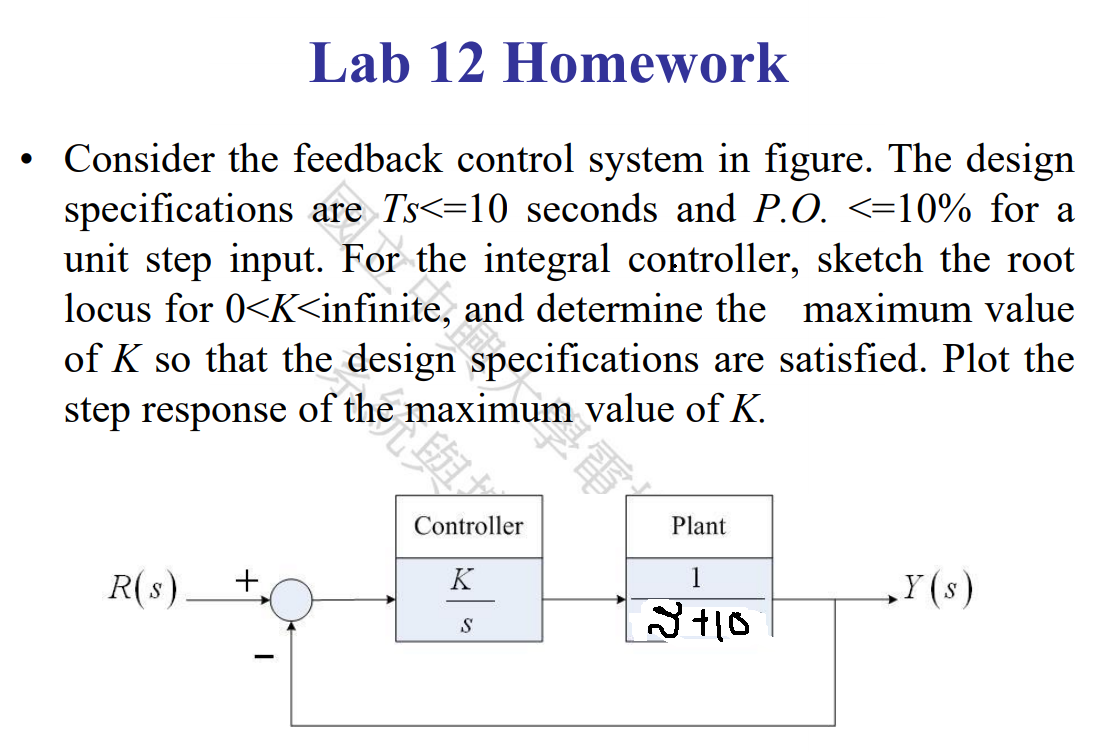
\includegraphics[scale=0.5]{../Lab12/Problem2.png}\\
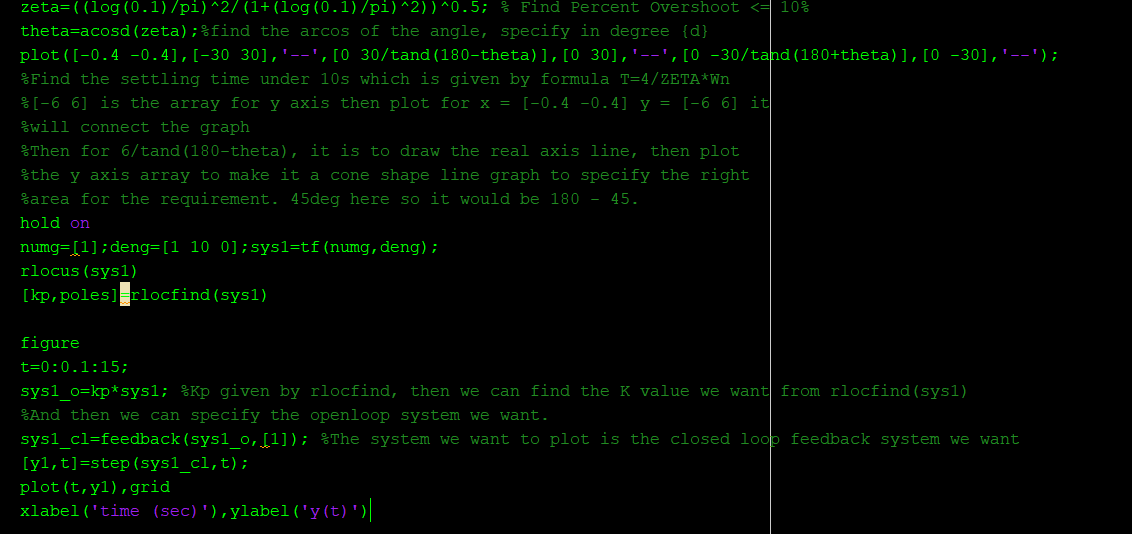
\includegraphics[scale=0.7]{../Lab12/Code2.png}\\ 

\cleardoublepage


\subsection{Plot Response OF the given systems with the desire K} 
The following is the systems out given\\

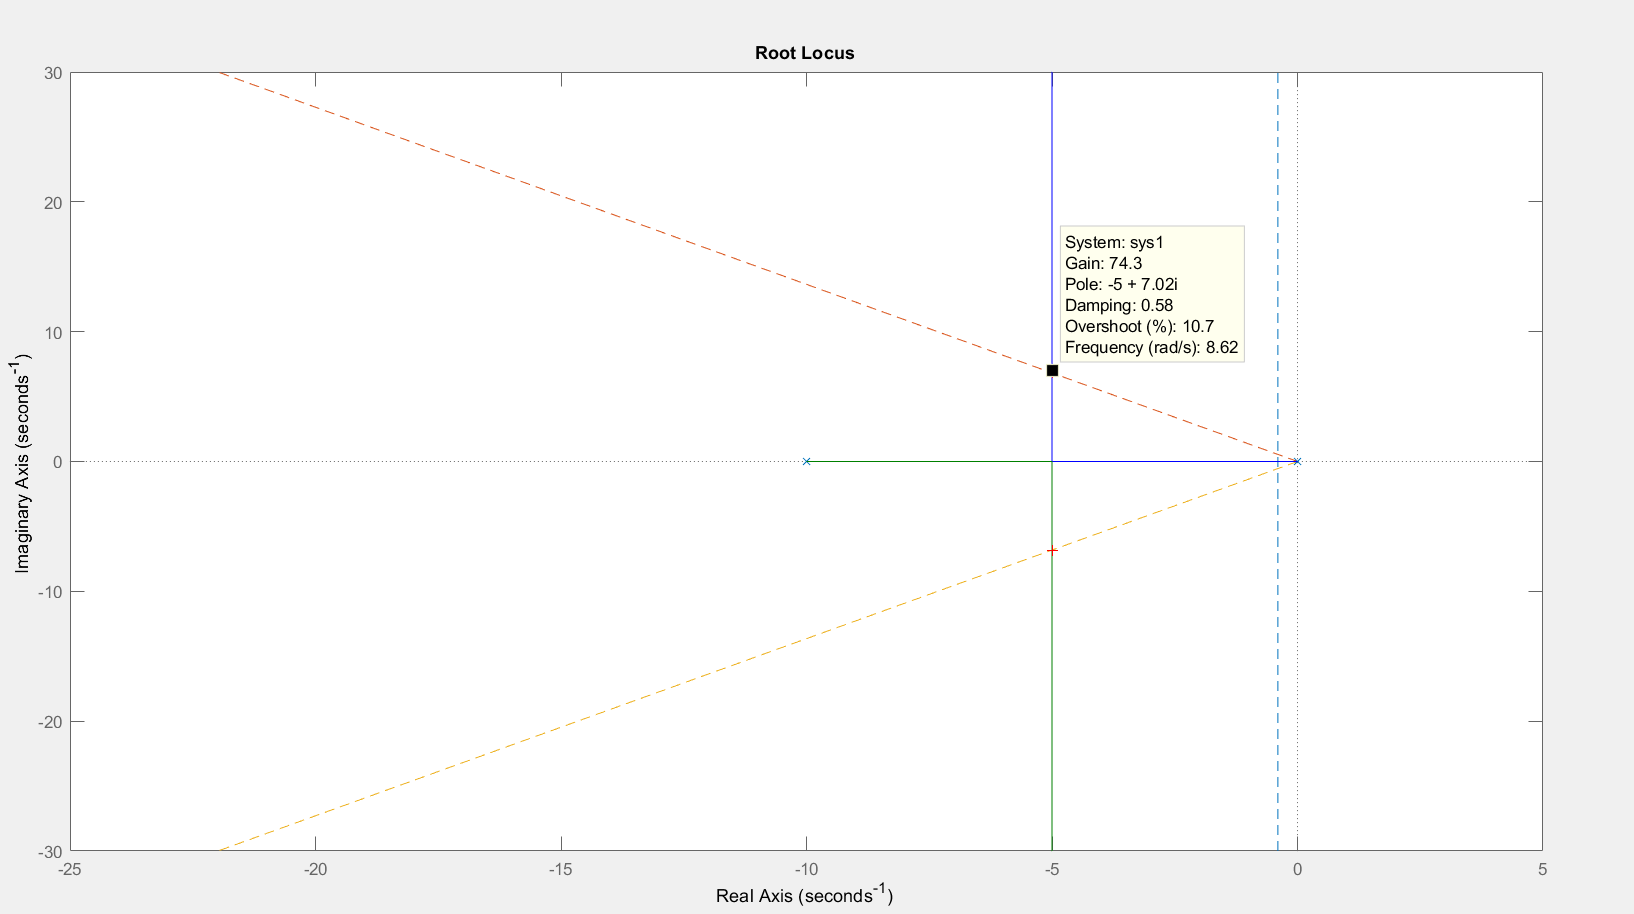
\includegraphics[scale=0.4]{../Lab12/Result2.png}\\

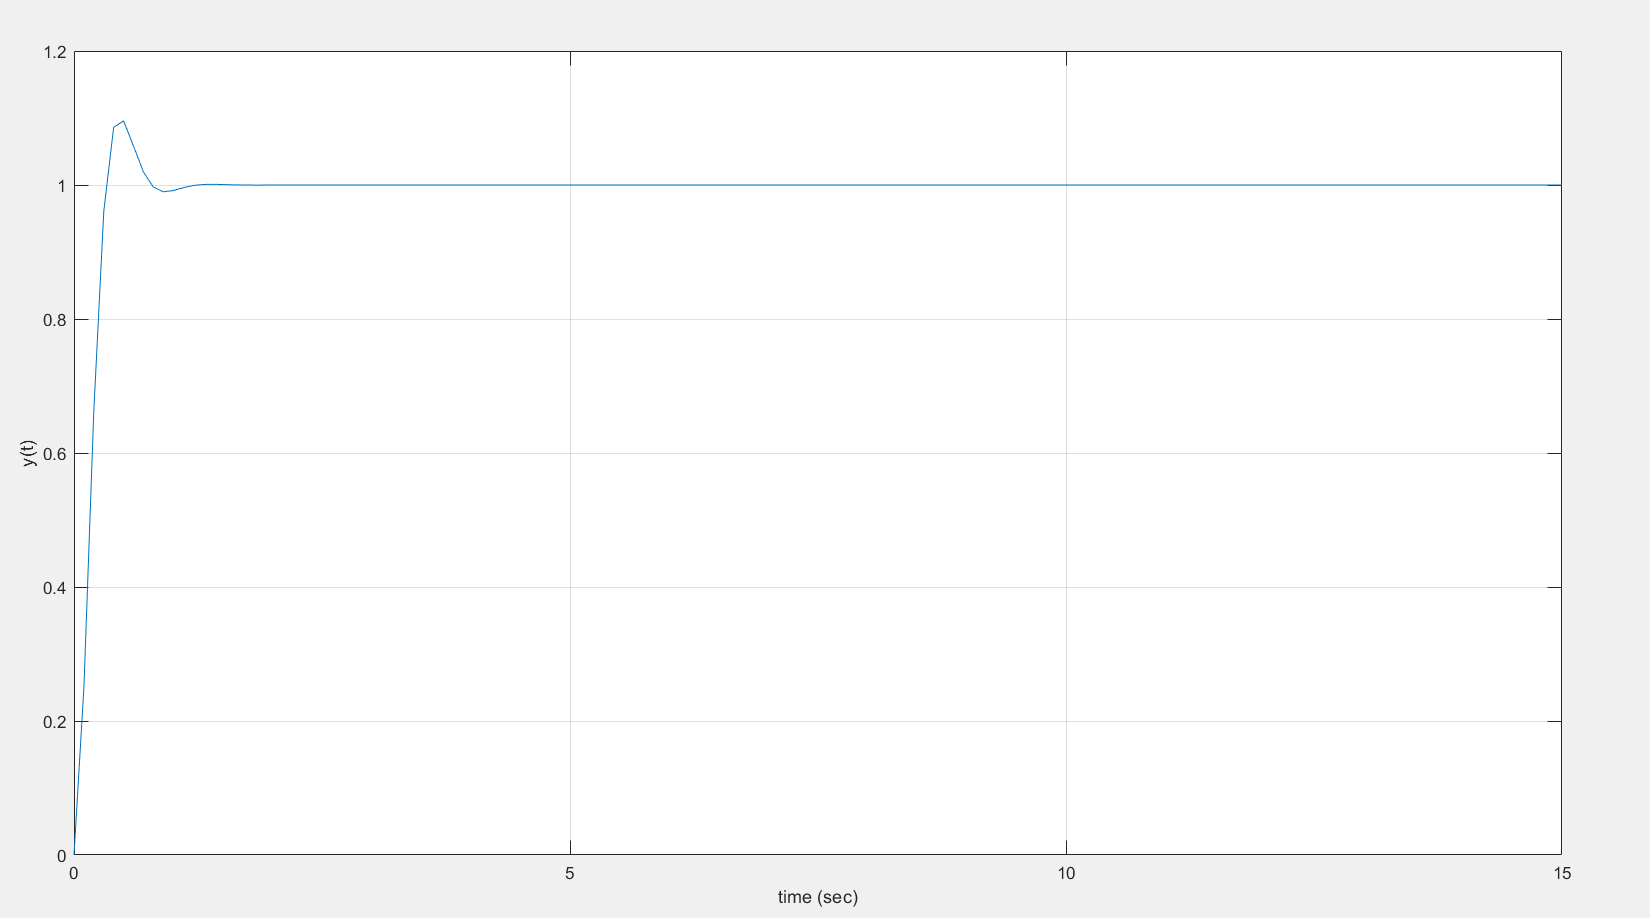
\includegraphics[scale=0.4]{../Lab12/Result2_Responses.png}\\ 


\section{Conclusion}
Today we learn the plot of root locus which shows the powerful utility of Matlab which enable us to bypass the complicated calculation with root locus, makes us be able to easily find the desired K for the system, thus keep the system under our desired design condition.

\begin{center} 
This concludes this Week's Auto Control LAB\\
\end{center}

\end{document} 
